\documentclass[12pt]{article}
\usepackage[a4paper,margin=23mm]{geometry}
\usepackage{amsmath,amssymb,booktabs,longtable,array,graphicx,microtype}
\usepackage[hidelinks]{hyperref}
\usepackage{url}
\setlength{\parindent}{0pt}
\setlength{\parskip}{5pt}
\setlength{\tabcolsep}{5pt}
\hypersetup{pdftitle={City Opportunities: Data and Evaluation},pdfauthor={}}
% Generated from frozen research outputs; do not hand-edit numerical claims.
\newcommand{\TotalWidthReduction}{13.97 }
\newcommand{\MethodComparison}{TOPSIS selects Zurich at the midpoint, whereas VIKOR selects Dublin; Kendall's $\tau_b=0.483$. Dublin satisfies VIKOR's advantage and stability conditions. Under equal weights, Oslo has the lowest VIKOR index but fails those acceptance conditions, so it is not an accepted unique compromise solution. }
\newcommand{\FutureDeterministic}{All three uniform-change scenarios retain Zurich as the conservative recommendation and all sixteen cities as possible champions under both weight references, including the Singapore-proxy withdrawal arm. Balanced improvement changes the fixed-weight second and third decisions from Singapore--Oslo to Oslo--Singapore. }
\newcommand{\FutureThresholds}{Oslo reaches the tie at approximately 5.685\% reduction, Singapore at 10.309\%, and Stockholm at 28.875\%. Zurich already minimizes regret at baseline. A slightly greater reduction produces a strict recommendation switch in these calculations. }
\newcommand{\FutureMonteCarlo}{Specifically, $C\sim U[0,1]$ is shared across cities and $I_i\sim U[0,1]$ varies by city, independently; $\delta_i=0.05C+0.05I_i$. The relevant raw multipliers are $1+\delta_i$ or $1-\delta_i$, and affected criteria within a city share that multiplier. With 10,000 draws per scenario, Zurich's fixed-weight recommendation frequencies are 100.00\%, 96.85\%, 97.72\% for resource expansion, living pressure and balanced improvement respectively. }
\newcommand{\PreferenceResults}{Education priority changes the conservative recommendation from Zurich to Oslo, with decision-rank $\tau_b=0.700$ relative to baseline. Independent-living priority retains Zurich and gives $\tau_b=0.917$. All sixteen cities remain possible champions in each profile. }
\newcommand{\MonteCarloInterpretation}{At concentration 100, Oslo has a better mean decision rank (2.1062) than Zurich (2.2305), although Zurich has the greater recommendation frequency and is the fixed-weight minimax choice. At concentration 20 under education priority, Singapore is the most frequently recommended city, whereas the fixed education-priority decision is Oslo. }
\newcommand{\EquityCase}{A separate Shanghai school-resource case uses 16 districts, 235,542 regular senior-secondary pupils and 23,999 full-time teachers in the 2025 school year. The pooled utility is 0.604481; the student-weighted mean of district utilities is 0.603267. Ordering districts by resource utility and averaging the bottom 20\% of pupil mass, with fractional inclusion of the boundary district, gives 0.580954, 0.022313 below the weighted mean. These are district-homogeneous school-location resource scenarios, not observed individual teacher exposure or resident accessibility \cite{shanghai}. }
\newcommand{\AgeCase}{A historical Istanbul household survey offers current-high-school groups aged 14--15 and 16--18. Their travel-utility marginal bounds overlap: $[0.35961,0.55711]$ and $[0.29347,0.59346]$, respectively. They include unknown durations and optional members; shared unknown-age mass means their extrema need not be jointly attainable. They describe 2012 broad groups, not exact ages fourteen and eighteen today. Singapore's MOE table records 38,555 students aged fourteen and only 165 aged eighteen at the start of 2020 still in secondary schooling; the latter is not an all-eighteen-year-old resident denominator. These counts cannot be joined to census school-stage travel bins without a matching population/reference-day table \cite{istanbul,sgage}. }
\newcommand{\CountryInterpretation}{Phoenix has higher retained affordability utilities than New York. Mumbai has the higher PM$_{2.5}$ utility, while Delhi has higher living-cost, housing, school-resource and broadband utilities in the retained evidence. The cases inherit the historical study's geographic and educational scope; their score pairs overlap, so neither case identifies a necessary overall winner. }
\newcommand{\CaseReferences}{\bibitem{shanghai} Shanghai Municipal Education Commission. Regular secondary-school pupil and teacher tables, school year 2025. \url{https://edu.sh.gov.cn/xxgk2_zhzw_tjsj_01/20260610/890926a33cbf443d9abf07c6f65b7734.html}. \bibitem{istanbul} Istanbul Metropolitan Municipality. 2012 household transport survey, official data-portal response resource \texttt{a75118db-28c9-4fdf-b367-d5933b7bb810}; questionnaire, report and nonidentifying aggregate audit archived. \bibitem{sgage} Singapore Ministry of Education. Secondary enrolment by level and age, 2020. \url{https://data.gov.sg/datasets/d_cc84fc751ef5106d9e26cfdbf61776c8/view}. }

\title{City Opportunities: Data, Evaluation and Model Extension}
\author{}
\date{}
\begin{document}
\maketitle
\noindent Evidence-based bounds support a conservative city recommendation while
retaining missing observations. In the sixteen-city comparison, verified
supplementation narrows average score intervals by \TotalWidthReduction\%.
Zurich minimizes maximum regret under the baseline weights, while all sixteen
cities remain possible champions.

\setcounter{section}{3}
\section{Data collection and comparability}
\subsection{A traceable city--indicator matrix}
We compare $M=16$ cities on $N=10$ indicators covering safety, environment,
household costs, education and everyday resources. The initial matrix is the
team-supplied city table \cite{teamtable}. We retain its existing values, populations, reference
years and source flags as the agreed input, then supplement only empty cells.
Some supplied values lack original source URLs, so their provenance remains
the team table; official supplements do not retrospectively validate every
supplied measurement. Table~\ref{tab:indicators} states what each variable measures.

\begin{longtable}{p{.22\linewidth}p{.56\linewidth}r}
\caption{Retained indicators, units and reference anchors. Supplied values are retained; supplements have explicit source scope.}\label{tab:indicators}\\
\toprule Indicator & Measurement and interpretation & Anchor\\\midrule
\endfirsthead
\toprule Indicator & Measurement and interpretation & Anchor\\\midrule\endhead
Homicide & Deaths per 100,000; cost; supplied city proxy & 2 \\
PM$_{2.5}$ & $\mu$g/m$^3$; cost; supplied concentration proxy & 15 \\
Living costs & Supplied living-cost index; cost & 100 \\
Housing & Supplied price-to-income ratio; cost & 10 \\
School resources & Pupils per teacher or explicitly scoped FTE; cost & 15 \\
Higher education & Institutions per 100,000; benefit; supply proxy & 1 \\
Transport stops & Unique stops per 100,000; benefit; partial inventories & 50 \\
Travel & Duration in minutes; $\exp(-t/30)$; commute or stage proxy & 30 min \\
Broadband & Supplied Mbps; benefit; city/general-use proxy & 100 \\
Swimming pools & Venues per 100,000; benefit; supply proxy & 1 \\
\bottomrule
\end{longtable}


The nominal reference year is 2025, but the evidence is mixed-vintage. Every
supplement retains its actual year rather than being relabelled as 2025.
Population denominators remain those of the supplied table. Thus a 2026 facility
snapshot divided by a supplied 2025 population is a conditional density, not an
observed same-year census. We do not infer that facilities are unchanged merely
because they may change slowly. Historical inventory assumptions are evaluated
through withdrawal scenarios.

We use official statistical tables, operator inventories and municipal geodata
to fill missing fields. For each admitted supplement, the archive records the
provider, URL, year, geographic and population scope, units, extraction rule and
file hash. Original PDFs and API responses are retained separately from derived
tables. Search summaries locate evidence; numerical admission requires the
underlying record or an explicitly identified provider capture. Values are
converted to compatible units before utility calculation: for example, the
supplied higher-education density per million is divided by ten to obtain the
per-100,000 scale. Mode share is not converted into physical stop density.

\subsection{Collection problems and their resolution}
\textbf{A station is not a platform, and a network is not a city.}
Oslo's municipal GIS represents platforms. Selecting records within the city
boundary and consolidating names gives 89 metro stations from 186 platforms.
Zurich's official 2025 VBZ report separately lists 446 stops on city territory
and 235 in the surrounding area; only 446 enter the city inventory
\cite{oslo,vbz}. A November 2026 snapshot of Helsinki's operator similarly
distinguishes 19 metro stations in Helsinki from 11 in Espoo \cite{helsinki}.
These are mode or operator subsets, so they supply
lower bounds rather than complete all-operator totals. For a verified facility
count $c$ and fixed population $P$, density is $d=10^5c/P$; utility is bounded by
$[d/(a+d),1]$.

\textbf{A list of venues can contain closed facilities.}
Stockholm's current municipal swimming directory lists fourteen named venues,
one of which is explicitly closed for renovation. The thirteen retained venues
agree with the current overview; the temporary year-round replacement is
counted once \cite{stockpool}. We count venues, not individual basins. This
municipal subset gives a supply lower bound and leaves other providers unknown.
Its access date is November 2026; a page-footer date is not used to reconstruct
a 2025 inventory. Paris's 244 intra-muros metro stations come from a March 2022
atlas using RATP 2021 and Apur 2022 sources, not a 2025 observation
\cite{apur}. A separate withdrawal restores this historical supplement to unknown.

\textbf{Pupils and teachers must refer to the same schools and stage.}
Prague's 2024/25 tables report 80,073 secondary-school pupils and 6,877.1
teacher full-time equivalents (FTE), including lower-gymnasium years.
Subtracting the matching 8,748 pupils and 737.8 FTE yields 71,325 pupils and
a rounding envelope of $[6139.2,6139.4]$ FTE \cite{prague}. The Prague
measure includes all study modes, including adult and non-daytime cohorts.
Stockholm's
published city-school ratio covers upper-secondary years 1--3 and all provider
ownership types, measured on 15 October \cite{kolada}. Its API value
16.42091405 is conservatively represented by $[16.35,16.45]$, an intentional
precision convention rather than a claimed measurement-error confidence interval.
In contrast, Paris's 72,476 lyc\'ee pupils cannot be divided by its 15,940
second-degree teachers because the teacher total includes coll\`eges
\cite{parisedu}; that missing ratio remains unknown. FTE resource measures
and school-location populations are distinguished from teacher headcounts and
resident high-school outcomes.

\textbf{Unavailable records and unobserved travellers are retained honestly.}
An initial Singapore census PDF endpoint returned 404; the official Parliament
mirror and official data API supplied the report and matching table
\cite{singapore}. Duration bins are converted using utility at their endpoints,
without bin midpoints or an artificial maximum duration for the open tail.
The stage-specific total enrolment estimates exceed the travel-table estimates
by estimated uncovered student totals of 1,811 for secondary, 989 for
post-secondary non-tertiary and 1,635 for polytechnic. These are weighted
survey estimates rather than complete headcounts. The uncovered mass retains
utility $[0,1]$; unknown stage proportions are
handled by the interval convex hull. The resulting $[0.21048,0.61884]$ is a
2020 school-stage proxy, not an identified 2025 interval for ages 14--18.
When Dublin raw stop downloads returned 403, no count was inferred from the
catalogue. A later official map supported a separately documented subset of
19 existing city-centre tram stops \cite{dublin}. A timed-out Warsaw school-travel download
was discarded and the field left unknown. Failed retrieval does not create a
numerical observation.

The current 160 cells comprise 112 point values, 27 partial intervals and
21 fully missing intervals. The original table had 112 points, 12 partial
intervals and 36 fully missing cells. The fifteen supplements therefore improve
information without replacing the team's existing measurements. Facility supply,
general commute proxies and school resources remain distinct from adolescent
access, school travel and learning quality.

\section{Establishing the baseline evaluation model}
\subsection{Determining indicator weights}
We retain eight main indicators at weight 0.1125 each and two auxiliary facility
indicators, transport stops and pools, at 0.05 each, so $\sum_jw_j=1$.
These weights express a transparent modelling choice. They are not estimated
from a student survey. Equal weights provide a separate reference.
TOPSIS is the primary score; VIKOR provides a focused method comparison.
AHP represents explicit preference scenarios \cite{saaty}, and Monte Carlo measures
sensitivity to declared distributions. These extensions retain the same
criteria rather than introduce unrelated ranking models.

For preference multipliers $m_j>0$, we use
\begin{equation}
 w'_j=\frac{m_jw_j}{\sum_kw_km_k},\qquad A_{jk}=\frac{w'_j}{w'_k}.
 \label{eq:weights}
\end{equation}
The principal eigenvector of $A$ recovers $w'$. With $\lambda_{\max}$ its
largest eigenvalue, $CI=(\lambda_{\max}-N)/(N-1)$ and $CR=CI/RI_N$.
Because this matrix is built from exact ratios, $\lambda_{\max}=N$ and
$CR=0$ up to numerical precision. This verifies internal consistency;
it does not establish that these are students' actual preferences.

\subsection{TOPSIS scoring calculation}
We adapt TOPSIS \cite{topsis} using fixed reference anchors to preserve a common scoring scale across evidence,
preference and future scenarios. For benefit and cost measurements respectively,
\begin{equation}
 u^{+}(x)=\frac{x}{a+x},\qquad u^{-}(x)=\frac{a}{a+x}.
\end{equation}
Each anchor in Table~\ref{tab:indicators} is a declared reference scale, not
an estimated optimum. Travel uses $q(t)=e^{-t/30}$ for duration $t$ in minutes.
When only mean duration $\bar t$ is known, Jensen's inequality gives
$\mathbb E[q(t)]\in[e^{-\bar t/30},1]$. Fully missing utilities remain $[0,1]$.

For utility vector $u_i$, weighted distances from fixed worst and best points are
\begin{equation}
 D_i^-=\sqrt{\sum_jw_ju_{ij}^2},\qquad
 D_i^+=\sqrt{\sum_jw_j(1-u_{ij})^2},\qquad
 S_i=100\frac{D_i^-}{D_i^-+D_i^+}.
\end{equation}
Weights enter the squared distances once. Since $S_i$ increases with every
utility, endpoints $\ell_i,h_i$ give $L_i=S(\ell_i)$ and $U_i=S(h_i)$.
Under the retained rectangular uncertainty set, define
\begin{equation}
 R_i=\max\{0,\max_{k\ne i}U_k-L_i\},\qquad
 i^*\in\arg\min_iR_i,
 \label{eq:regret}
\end{equation}
\begin{equation}
 \mathcal C=\{i:U_i\geq\max_{k\ne i}L_k\}.
\end{equation}
Maximum regret $R_i$ measures how far the selected city could trail another
city. Set $\mathcal C$ retains every city that could still be first.
The maximum excludes the selected city itself. These conditional data bounds
are not sampling confidence intervals, and a conservative recommendation does
not identify a uniquely best city.

\subsection{Scoring results and interpretation}
Zurich minimizes maximum regret, followed by Singapore and Oslo
(Table~\ref{tab:baseline}). Zurich's score lower bound is below those of
Singapore and Oslo; its own upper bound is excluded from its competitor set.
Its regret is $70.90353-53.53548=17.36805$, whereas Oslo's is
$72.18379-54.29594=17.88785$. All sixteen cities remain possible champions.
The decision order expresses a conservative recommendation under the stated
criteria and intervals.

\begin{longtable}{rlrr}
\caption{Conservative baseline decision ranks with unchanged weights.}\label{tab:baseline}\\
\toprule Rank & City & Score interval & Maximum regret\\\midrule
\endfirsthead
\toprule Rank & City & Score interval & Maximum regret\\\midrule\endhead
1 & Zurich & 53.54--72.18 & 17.37 \\
2 & Singapore & 54.33--63.53 & 17.85 \\
3 & Oslo & 54.30--63.90 & 17.89 \\
4 & Stockholm & 52.12--64.54 & 20.06 \\
5 & Prague & 51.62--62.78 & 20.56 \\
6 & Dublin & 51.13--70.90 & 21.05 \\
7 & Berlin & 50.49--61.54 & 21.69 \\
8 & Helsinki & 49.41--69.84 & 22.78 \\
9 & Paris & 49.11--69.04 & 23.08 \\
10 & Madrid & 48.63--68.22 & 23.56 \\
11 & Warsaw & 47.50--63.99 & 24.69 \\
12 & Vienna & 47.19--61.03 & 25.00 \\
13 & Milan & 45.63--65.99 & 26.56 \\
14 & London & 45.17--66.12 & 27.01 \\
15 & Tokyo & 43.81--61.12 & 28.38 \\
16 & Amsterdam & 42.29--60.43 & 29.90 \\
\bottomrule
\end{longtable}


\begin{figure}[htbp]
\centering
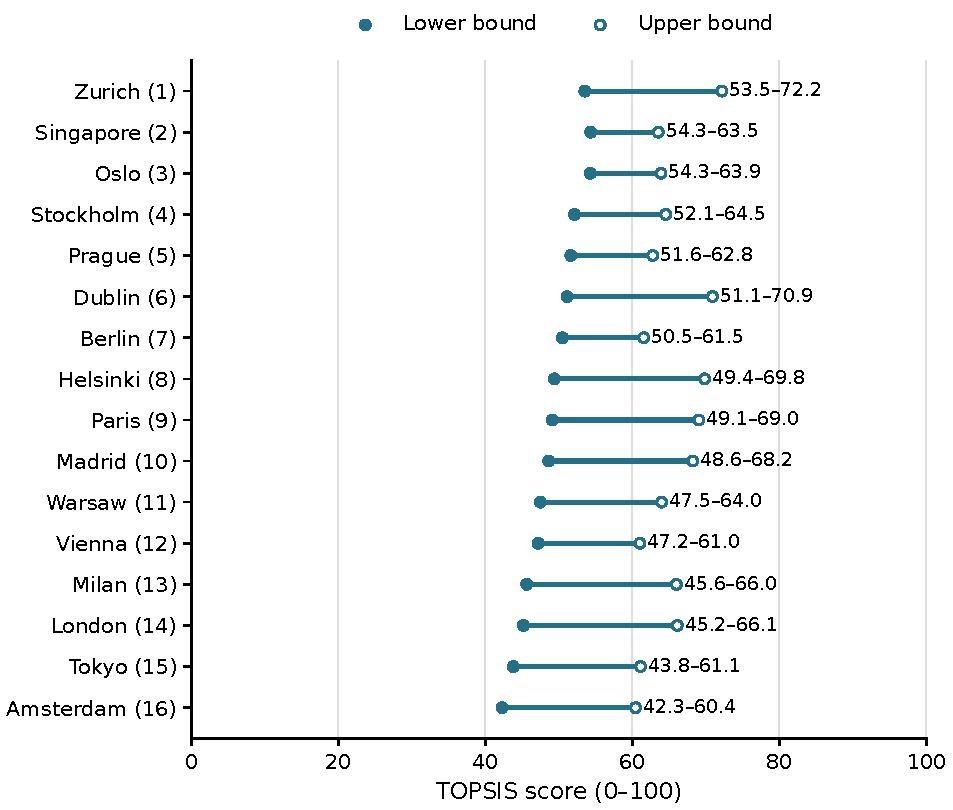
\includegraphics[width=\linewidth]{task4_v122_assets/score_intervals.pdf}
\caption{Current score bounds and conservative decision order for the sixteen
cities. Intervals retain missing information; they are not confidence intervals.
Source: frozen city matrix and admitted supplements.}
\label{fig:intervals}
\end{figure}

Holding weights and formulas fixed, the fifteen admitted supplements narrow
the average fixed-weight score interval from 18.81077 to 16.18302, a
\TotalWidthReduction\% reduction. The most recent five additions alone narrow
it by 4.44\%, moving Stockholm from thirteenth to fourth. Withdrawal of the
two recent historical transport inventories still recommends Zurich; withdrawal
of Singapore's historical school-stage travel proxy also preserves this
recommendation. Evidence improves precision and changes decisions before it
necessarily reduces the possible-champion set.

As a method diagnostic, TOPSIS and VIKOR use the same illustrative midpoint
utilities and weights. VIKOR balances total and largest weighted shortfalls
equally and uses sample best/worst values \cite{vikor}. \MethodComparison
The midpoint comparison does not replace the interval decision in
Equation~\ref{eq:regret}. Agreement indicates similarity within the chosen
conventions; disagreement exposes method dependence rather than justifying a
post-hoc choice of the preferred winner.

\section{Model revision and extension}
\subsection{Considering future changes}
We examine three conditional changes while holding anchors and population
denominators fixed. Resource expansion raises higher-education, stop and pool
densities by 10\%. Living pressure raises living costs, housing cost ratios and
travel durations by 10\%. Balanced improvement reduces pupil--teacher ratios,
PM$_{2.5}$ and travel durations by 10\%. A comparable multi-year panel is not
available, so these changes have no estimated annual rate or forecast date.

For raw multiplier $r>0$, the utility transformations are
\begin{equation}
 T_r^{+}(u)=\frac{ru}{1-u+ru},\qquad
 T_r^{-}(u)=\frac{u}{u+r(1-u)}.
\end{equation}
These increasing maps propagate raw-scale changes through benefit and cost
intervals. For known mean travel duration, the new Jensen interval is
$[e^{-r\bar t/30},1]$. Singapore instead has bounds $[L_q,U_q]$ on expected
utility. With $q=e^{-t/30}$ and $t'=rt$, Jensen and $0\leq q\leq1$ give
\begin{equation}
 \mathbb E[q^r]\in
 \begin{cases}
 [L_q,U_q^r],&0<r<1,\\
 [L_q,U_q],&r=1,\\
 [L_q^r,U_q],&r>1.
 \end{cases}
 \label{eq:moment}
\end{equation}
Raising both endpoints to $r$ would generally misrepresent an expected utility.
Equation~\ref{eq:moment} is an outer moment bound and need not be reversible.
Fully missing travel remains unknown. Thus the extension accommodates the
different information supplied by means and by travel distributions.

\FutureDeterministic
We also solve a decision boundary: holding other cities fixed, proportionally
reduce one city's pupil--teacher ratio, PM$_{2.5}$ and travel durations until
its maximum regret ties that of the best other city. \FutureThresholds
These thresholds describe the model response to a specified joint change;
they do not establish policy feasibility or a uniquely identified champion.

For a separate future-shock simulation, each draw combines a common shock and
city-specific shocks under a declared bounded distribution, with the criterion
weights held fixed. Original data intervals are not randomly completed.
\FutureMonteCarlo
These are conditional stress frequencies under an uncalibrated distribution.
Weight perturbations below answer a separate question and are not blended
silently into the future-shock frequencies.

\subsection{Considering different preferences and development situations}
Education priority doubles the weights of the two education indicators.
The independent living scenario doubles travel and transport-stop weights.
Equation~\ref{eq:weights} then normalizes all weights.
\PreferenceResults
The resulting differences show how the definition of a desirable city affects
the decision. They do not establish measured differences between fourteen- and
eighteen-year-old students.

\subsection{Perturbing weights}
For each preference centre $w'$, we draw
$w^{(b)}\sim\operatorname{Dirichlet}(\kappa w')$, with
$\kappa\in\{20,100,500\}$ and 10,000 draws per setting. Every draw recomputes
interval TOPSIS and maximum regret without filling missing values. We report
mean decision rank, fractional first-place recommendation frequency and
fractional top-three decision membership; ties share membership.

\begin{table}[htbp]\centering
\caption{Conditional recommendation frequencies (\%) at concentration 100.}
\begin{tabular}{lrrr}\toprule Preference centre & Zurich & Oslo & Singapore\\\midrule
Baseline & 43.34 & 28.00 & 28.23 \\
Education priority & 6.83 & 45.62 & 42.11 \\
Independent living & 58.99 & 15.46 & 25.12 \\
\bottomrule\end{tabular}\end{table}


\begin{figure}[htbp]
\centering
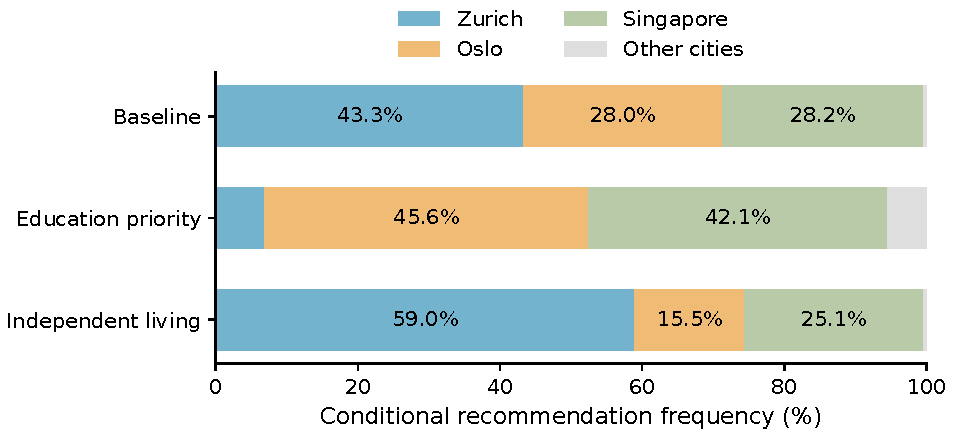
\includegraphics[width=\linewidth]{task4_v122_assets/preference_frequencies.pdf}
\caption{Recommendation frequencies under three declared preference centres,
Dirichlet concentration 100 and 10,000 draws per centre. Frequencies are conditional
on analyst-selected weight distributions, not probabilities of true superiority.
Source: unchanged city evidence and declared preference multipliers.}
\end{figure}

\MonteCarloInterpretation
These two summaries optimize different quantities. We retain minimum maximum
regret as the predeclared decision rule; Monte Carlo reports its sensitivity.
Neither average ranks nor a network aggregation resolves the missing empirical
information. A low AHP consistency ratio and repeated simulations demonstrate
calculation properties, not representative student opinion.

\subsection{Within-city fairness and growth stages}
Citywide facilities per resident measure supply, not who can use it. Fees,
opening hours, transport links, disability access and neighbourhood location
can separate nominal supply from student opportunity. Without matched student
locations and qualifying facilities, the city-level matrix cannot identify
these access distributions.

\EquityCase
To extend the same education criterion to districts $d$, let $n_d$ be the
matched pupil count and $r_d$ its pupil--teacher ratio. The student-weighted
utility is $\bar u=\sum_d n_d\,15/(15+r_d)/\sum_dn_d$.
Its difference from a citywide ratio reflects spatial aggregation, not an
effect of any particular policy. A school-location analysis also does not locate
resident students or establish their travel access.

For future access measurement, define $a_s$ as a student's qualifying access
measure, incorporating the relevant eligibility, price and time conditions.
With student weights $p_s$, report the weighted mean and the bottom-20\%
mean using fractional inclusion at the threshold. A common safety or travel
standard could also be reported as weighted coverage. These require additional
matched data; substituting a municipal average would not measure fairness.

\AgeCase
We therefore separate two mechanisms: age can change the observed indicators
(travel, permissions or opportunities), and preferences can change the weights.
An evidence-based age comparison would require $u_{ij}^{(14)}$ and
$u_{ij}^{(18)}$ for comparable residents, then independently elicited
$w_j^{(14)}$ and $w_j^{(18)}$ where available. The present preference scenarios
test priorities without assigning unsupported age labels or pretending that
all students face the same access.

\section{Comparing cities within the same country}
Every primary city belongs to a different country, so the main sample cannot
identify within-country city contrasts. We use the existing United States and
India cases as separately versioned examples with the same ten indicator
definitions and scoring formula. They do not enter the sixteen-city ranking,
and comparison within a country does not remove differences in source year,
city boundary or educational coverage.

\begin{table}[htbp]\centering
\caption{Separate historical country cases using the legacy 25-city V117 evidence.}
\begin{tabular}{llr}\toprule Country & City & Score interval\\\midrule
United States & Phoenix & 31.39--71.68 \\
 & New York & 30.22--72.81 \\
India & Mumbai & 28.82--60.64 \\
 & Delhi & 32.59--63.90 \\
\bottomrule\end{tabular}\end{table}


\CountryInterpretation
Overlapping score intervals leave both cities possible winners within each
pair. Dimension-specific differences are more informative than attributing
every score difference to a national effect. No causal national explanation is
identified by these descriptive cases.

\section*{Reproducibility and integration note}
The research archive preserves the unchanged team CSV, admitted-source hashes,
utility bounds, ranking tables, scenario multipliers and simulation seeds.
The frozen primary evidence version is V121; the current extensions are V122.
Historical country and district/age cases retain their own versions and scope.
Independent checks reproduce the score formula, competitor self-exclusion,
recommendation frequencies and relevant transformation bounds. The source
manifest records original files separately from derived extracts.

This document is a standalone chapter contribution, not a complete contest
submission. The shared manuscript, summary sheet, news article, complete
references and AI-use report require their own integration and final review.

\begin{thebibliography}{20}
\raggedright
\bibitem{teamtable} Team-supplied city-indicator table, sixteen cities.
Frozen input archived November 2026; original values, years and flags retained.
\bibitem{saaty} T. L. Saaty. The analytic hierarchy process---what it is and
how it is used. \textit{Mathematical Modelling}, 9(3--5), 161--176, 1987.
\url{https://doi.org/10.1016/0270-0255(87)90473-8}.
\bibitem{topsis} C.-L. Hwang and K. Yoon. \textit{Multiple Attribute Decision
Making: Methods and Applications}. Springer, 1981.
\url{https://doi.org/10.1007/978-3-642-48318-9}.
\bibitem{vikor} S. Opricovic and G.-H. Tzeng. Compromise solution by MCDM
methods: A comparative analysis of VIKOR and TOPSIS.
\textit{European Journal of Operational Research}, 156(2), 445--455, 2004.
\url{https://doi.org/10.1016/S0377-2217(03)00020-1}.
\bibitem{oslo} City of Oslo, municipal transport GIS, layer 800; Norwegian
Mapping Authority, municipality 0301 boundary. Accessed November 2026.
\url{https://geodata.bymoslo.no/arcgis/rest/services/geodata/Temadata_Publikum/MapServer/800}.
\bibitem{vbz} Verkehrsbetriebe Z\"urich. \textit{Zahlen und Fakten 2025}, p.~6.
\url{https://www.stadt-zuerich.ch/content/dam/vbz/de/die-vbz/zahlen-fakten/geschaeftsbericht/Z4690_VBZ_FB-2025_Web.pdf}.
\bibitem{helsinki} Metropolitan Area Transport Ltd. \textit{Metrolla}.
Official operator inventory, accessed November 2026.
\url{https://kaupunkiliikenne.fi/liikennointi/metrolla/}.
\bibitem{stockpool} City of Stockholm. \textit{Simhallarna} and current swimming
overview. Accessed 8 November 2026.
\url{https://motionera.stockholm/trana-gymma-simma/simhallarna/}.
\bibitem{apur} Atelier parisien d'urbanisme. \textit{Atlas des activit\'es \`a
Paris}, March 2022, p.~37. Sources RATP 2021 and Apur 2022.
\url{https://www.apur.org/sites/default/files/atlas_activites_paris_immobilier.pdf}.
\bibitem{prague} Czech Statistical Office. \textit{Schools and school facilities,
2024/25}, Tables 3.1.3 and 6.1.18.
\url{https://csu.gov.cz/docs/107508/299702e7-bc0a-1dc2-87db-600d0303f2f4/23004225.pdf?version=1.1}.
\bibitem{kolada} RKA/Kolada, indicator N17816, Stockholm municipality 0180,
period 2025; source Skolverket (Siris). Definition and total-provider scope
archived with the API response.
\url{https://api.kolada.se/v3/data/kpi/N17816/municipality/0180/year/2025}.
\bibitem{parisedu} Acad\'emie de Paris. \textit{Chiffres cl\'es 2025},
2024 school-entry pupils and 31 December 2024 teacher totals.
\url{https://www.ac-paris.fr/sites/ac_paris/files/2025-08/chiffres-cl-s-acad-mie-de-paris-44994.pdf}.
\bibitem{singapore} Singapore Department of Statistics. \textit{Census of
Population 2020, Statistical Release 2}, Tables 93 and 124; official Parliament
mirror and official data API.
\url{https://www.parliament.gov.sg/docs/default-source/default-document-library/cop2020sr2.pdf}.
\bibitem{dublin} Dublin City Council and National Transport Authority.
\textit{Dublin City Centre Transport Plan 2023, Technical Note 6},
issued 2024, Figure 3-7.
\url{https://www.dublincity.ie/sites/default/files/2024-04/06-dublin-city-centre-transport-plan-public-transport-technical-note.pdf}.
\CaseReferences
\end{thebibliography}
\end{document}
